\documentclass[letterpaper]{article}

%% Language and font encodings
\usepackage[english]{babel}
\usepackage{fontspec}

%% Sets page size and margins
\usepackage[a4paper,top=2cm,bottom=2cm,left=2cm,right=2cm,marginparwidth=1.75cm]{geometry}

%% Useful packages
\usepackage{amsmath,amsthm,amssymb,amsfonts}
\mathchardef\mhyphen="2D
\usepackage{graphicx}
\usepackage[colorinlistoftodos]{todonotes}
\usepackage[colorlinks=true, allcolors=blue]{hyperref}
\usepackage{enumitem}
\usepackage{marginnote}
\usepackage{pgfplots}
\pgfplotsset{compat=1.13}
\usepackage{mathtools}
\usepackage[normalem]{ulem}
\usepackage[utf8]{inputenc}
\usepackage{fancyhdr}

\newcommand{\R}{\mathbb{R}}
\newcommand{\N}{\mathbb{N}}
\newcommand{\Z}{\mathbb{Z}}
\providecommand{\C}{\mathbb{C}}

\author{Henry Yu}

\renewcommand{\baselinestretch}{1.5}
\fancypagestyle{plain}{%
	\fancyhead[R]{\fbox{Varun Krishnamurthi, West Loden, Henry Yu}}
	\renewcommand{\headrulewidth}{0pt}
}

\title{Nauseating Ride Problem}

\date{}

\begin{document}
\maketitle

\hspace{3.8cm}
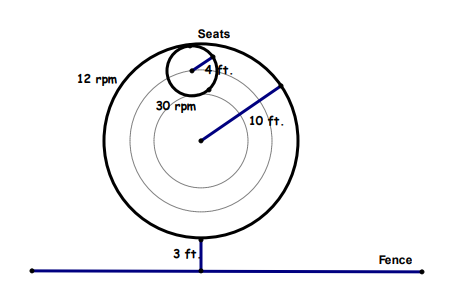
\includegraphics[scale=0.75]{graphhhh.png}

\section{}
Find your linear velocity in ft/s due to the combined rotation of the seats on the merry-go-round when you are:
\begin{itemize}
 \item farthest from the center.
 \item closest to the center. \vspace{6mm}

       $\cfrac{12 \hspace{1mm}rotations}{1 \hspace{1mm} minute}$ \times \hspace{1mm} $\cfrac{20\pi \hspace{1mm}feet}{1 \hspace{1mm}rotation}$ \times \hspace{1mm} $\cfrac{1 \hspace{1mm}minute}{60 \hspace{1mm}seconds}$ = 4$\pi$ \hspace{1mm}feet/second \hspace{3mm} (\text{larger circle [ merry-go-round ]}) \vspace{3mm}
       \\
       \newline
       $\cfrac{30 \hspace{1mm}rotations}{1 \hspace{1mm} minute}$ \times \hspace{1mm} $\cfrac{8\pi \hspace{1mm}feet}{1 \hspace{1mm}rotation}$ \times \hspace{1mm} $\cfrac{1 \hspace{1mm}minute}{60 \hspace{1mm}seconds}$ = 4$\pi$ \hspace{1mm}feet/second \hspace{3mm} (\text{smaller circle [ seat ]}) \vspace{3mm}
       \\
       \newline
       $\cfrac{12 \hspace{1mm}rotations}{1 \hspace{1mm} minute}$ \times \hspace{1mm} $\cfrac{12\pi \hspace{1mm}feet}{1 \hspace{1mm}rotation}$ \times \hspace{1mm} $\cfrac{1 \hspace{1mm}minute}{60 \hspace{1mm}seconds}$ = 2.4$\pi$ \hspace{1mm}feet/second \hspace{3mm} (\text{central circle}) \vspace{6mm}
       \\
       \newline
       Farthest = 8$\pi$ \hspace{1mm}\emph{feet/second} \text{ (counterclockwise)}
       \\
       \newline
       Closest = 1.6$\pi$ \hspace{1mm}\emph{feet/second} \text{ (clockwise)}
       \\

\end{itemize} \vspace{3mm}

\section{}

In what direction are you actually moving when your seat is closest to the merry-go-round’s
center? \vspace{3mm}

Based on the velocity of both circles, the seat would be moving clockwise since the velocity of the seat is greater than the central circle of the merry\mhyphen \text{go}\mhyphen \text{round}.
\section{}
Write the equation expressing your distance from the fence in terms of t. \vspace{3mm}

\underline {Addition of two cosine sinusoids}:

\noindent\begin{minipage}{0.45\textwidth}
\begin{align*}
y=6\cos\left(\frac{2\pi x}{5}\right)+4\cos\left(\frac{\pi x}{2}\right)+13
\end {align*}
\end{minipage}\hfill \vspace{3mm}

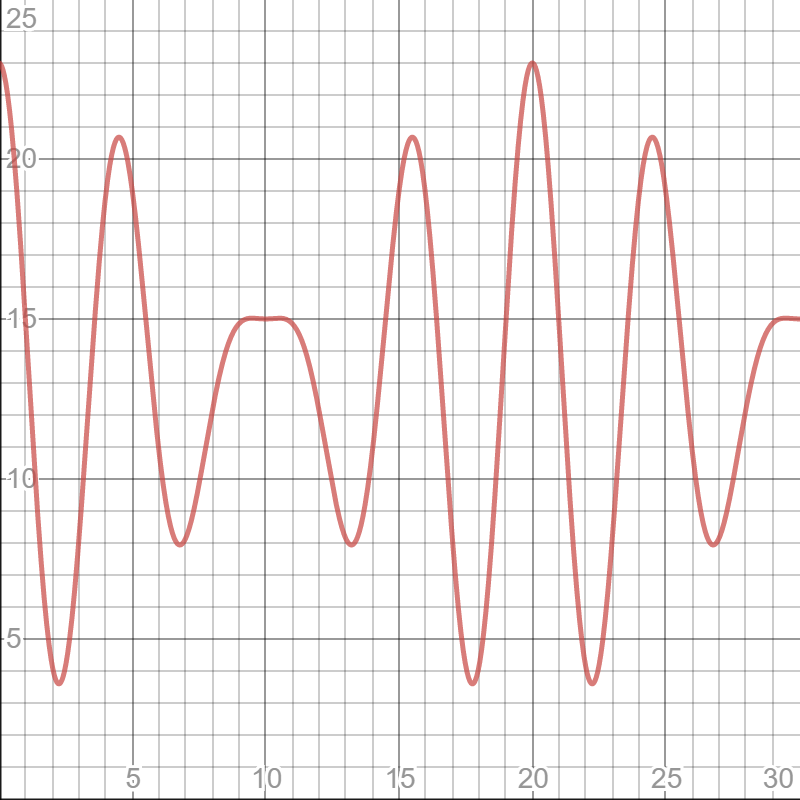
\includegraphics[scale=0.27]{desmos-graph (1).png} \vspace{3mm}


The whole function is an addition of two sinusoids. The bigger one has an amplitude of six feet (10 - 4) and has a period of 5 seconds (60$\hspace{1mm}$[$\cfrac{1}{12}$]$\hspace{1mm}$). The second graph has an amplitude of four feet and a period of two seconds (60$\hspace{1mm}$[$\cfrac{1}{30}$]$\hspace{1mm}$). Both graphs are cosine graphs, and the whole function has a vertical shift of thirteen feet (10 + 3). The period of the whole function is twenty seconds (2$\hspace{1mm}$[5\cdot 2]$\hspace{1mm}$).
\vspace{10mm}

Contributions:
Parts a and be were completed by West and verified by both other members, while parts c and d were completed by Varun. The document was compiled by Henry.
\\
\end{document}
